\chapter{Analysis and Discussion}
\label{ch07:discussion}
% Introduction to results - what were the experiment findings?
As demonstrated in Chapter \ref{ch06:results}, the Kafka Connect replication pipeline outperformed the Target Adapter even when no parallelization was implemented. The findings support the hypothesis outlined in Chapter \ref{ch05:methodology}, to the extent that leveraging parallelization had a positive impact on performance when compared to \ac{ART}. However, the additional predication that \ac{ART} would surpass Kafka Connect replication in single-threaded mode proved to be false. This chapter discusses the results and their implications in depth, and analyzes the effect of different factors on performance. In addition, areas where additional experiments or investigations could be performed are outlined to highlight areas requiring further research.

\section{Statistical Significance}
\label{ch07:discussion:statsig}
The confidence interval is used for determining the statistical significance of all average throughput measurements. It is also used to determine whether scenarios statistically differ from each other. The confidence level was set to 90\%, in accordance with the strategy outlined by \citeauthor{jain1991computer} \cite{jain1991computer}. The interval is typically inversely affected by the sample size and directly affected by variability and confidence level \cite{hazrausingci}. Since the sample size of five and confidence level are relatively low in the case of this experiment, any narrow intervals can most likely be attributed to low data variability. This will be regarded as true for all subsequent discussion. In the case of wide intervals, the same logic cannot be applied.

\subsection{Target Adapter}
The confidence interval for \ac{ART} is visualized in Figure \ref{fig:chapter07:discussion:artci}. The message throughput in Figure \ref{fig:chapter07:discussion:artavgmessageci} has error bars approximately between 1.91K and 1.96K, showing a relatively narrow interval. The narrow interval could be due to low variability in the measured data. The low variability is also supported by the small difference between the mean and median in Table \ref{tab:art:messagethroughput}.

Figure \ref{fig:chapter07:discussion:artavgtransci} shows the confidence interval for \ac{ART}'s total transaction throughput. It contains no visible bars, indicating that the interval is extremely narrow with only a 0.002 difference. This is supported by a very low standard error of 0.076 and no difference between the mean and median in Table \ref{tab:art:transactionthroughput}. A possible effect could be low data variability due to the throughput occurring in bursts instead of continually. This behavior will be elaborated upon in \ref{ch07:discussion:performancevariability}.

\begin{figure}[htbp]
    \centering
    \subfloat[Message throughput confidence interval]{\label{fig:chapter07:discussion:artavgmessageci}
        \centering
        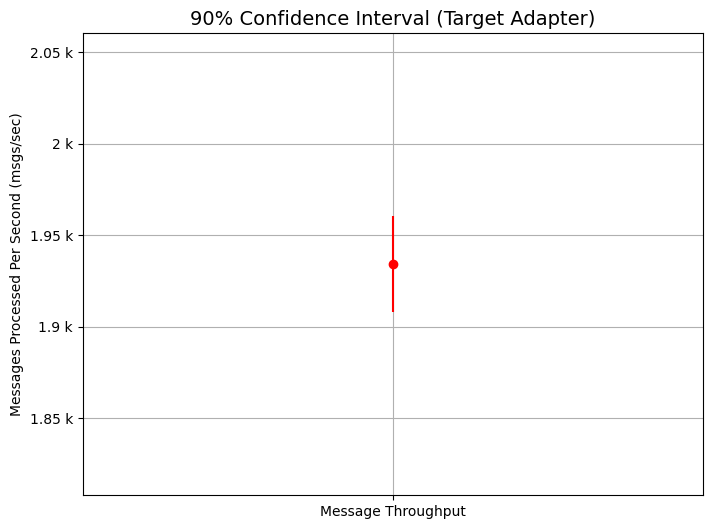
\includegraphics[width=0.75\textwidth]{chapters/images/confidence-intervals/art-message-ci.png}
    }
    \hfill
    \subfloat[Transaction throughput confidence interval]{\label{fig:chapter07:discussion:artavgtransci}
        \centering
        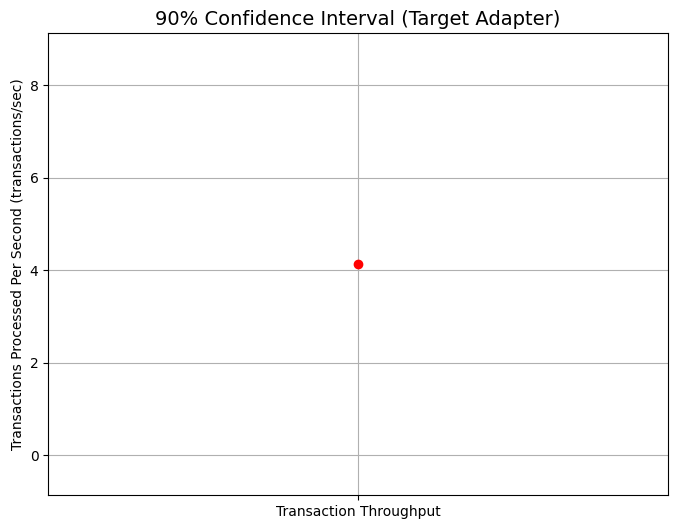
\includegraphics[width=0.75\textwidth]{chapters/images/confidence-intervals/art-transaction-ci.png}
    }
    \hfill
    \caption{Target Adapter throughput confidence interval}
    \label{fig:chapter07:discussion:artci}
\end{figure}

It was expected that \ac{ART} would perform approximately the same or even better compared to a single-threaded Kafka replication scenario. This expectation arose from the fact that \ac{ART} is monolithic and would not have any additional complexity arising from running multiple components, including latencies. However, this proved not to be the case. One possible explanation for that could be that the Kafka replication solution is more performant because it consumes binary messages instead of XML from the EntireX Broker. It would be interesting to compare the parsing performance of both solutions in future tests to determine whether that played a significant role or not. Another possible reason is that \ac{ART} supports transactionality to the complete extent, while in the Kafka-based solution only the source connector supports transactionality. It is possible that if the sink connector also had support for transactionality, that the total performance would be less than currently recorded. However, as the recorded performance of the source connector has shown in \ref{ch06:results:kafakreplicationperformance}, the source connector remained the most performant component of the entire pipeline despite its use of transactionality. Another possible investigation for future tests would be to explore the effect of transactionality on a source connector's and Kafka broker's performance.

\subsection{Source Connector}
The source connector's confidence interval for both the message and transaction throughput is visualized in Figure \ref{fig:chapter07:discussion:sourceci}. The interval for Scenario 1 in Figure \ref{fig:chapter07:discussion:sourcemessageci} is also too narrow to be seen, with bounds between approximately 26.3K and 27.8K. This could also be the result of low data variability. The rest of the scenarios also have relatively narrow intervals, with the widest interval being between 124K and 133K for Scenario 5. All scenarios are significantly different from each other based on a visual test of the confidence intervals \cite{jain1991computer}, with Scenario 2 and Scenario 3 only marginally passing that test.

\begin{figure}[htbp]
    \centering
    \subfloat[Message throughput confidence interval]{\label{fig:chapter07:discussion:sourcemessageci}
        \centering
        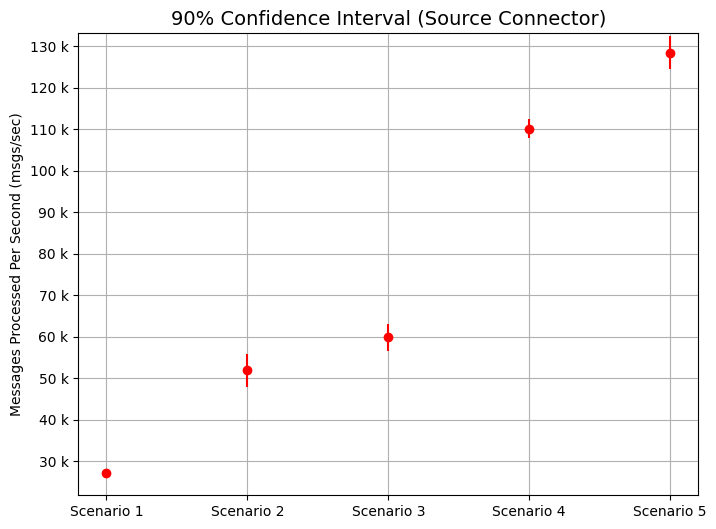
\includegraphics[width=0.75\textwidth]{chapters/images/confidence-intervals/source-message-ci.png}
    }
    \hfill
    \subfloat[Transaction throughput confidence interval]{\label{fig:chapter07:discussion:sourcetransci}
        \centering
        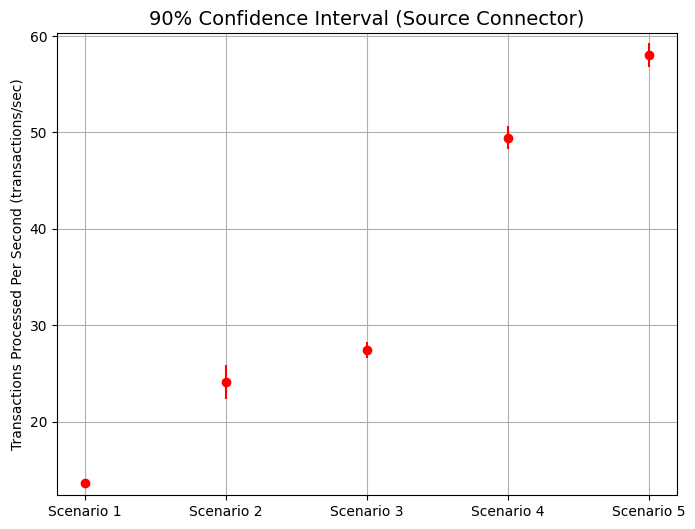
\includegraphics[width=0.75\textwidth]{chapters/images/confidence-intervals/source-transaction-ci.png}
    }
    \hfill
    \caption{Source connector throughput confidence interval}
    \label{fig:chapter07:discussion:sourceci}
\end{figure}

The confidence interval for the transaction throughput can be seen in Figure \ref{fig:chapter07:discussion:sourcetransci}. Just as in Figure \ref{fig:chapter07:discussion:sourcemessageci}, Scenario 1 has a small enough interval to not be visible on the visualization. The rest of the intervals have intervals of approximately 2-3 transactions in size. The largest interval was recorded in Scenario 2, with a bound between 22.4 and 25.8 transactions. The measurements in all scenarios are statistically different from each other, indicating a statistically significant increase in transaction throughput with each scenario.

\subsection{Broker}
The confidence interval for the broker's average message throughput can be found in Figure \ref{fig:chapter07:discussion:brokermessageci}. Scenarios 1 and 4 have no visible intervals, indicating a possibly low variation in the measured throughput. Scenario 5 has an uncommonly large interval between approximately 105K and 131K. It is unlikely for data variability to have played a role in this case, as the difference between the mean and median for Scenario 5 is not much different than for Scenario 4 in Table \ref{tab:kafka:messagethroughputbroker}, while the boundary size differs significantly. It is possible that the sample size of all runs to calculate the average of Scenarios 4 and 5 are too small, as the broker's activity duration was less than 1.5 minutes (see Figure \ref{fig:chapter06:results:brokerallscenarios}). This could have led to discrepancies in the estimation and standard error.

\begin{figure}[htbp]
    \centering
    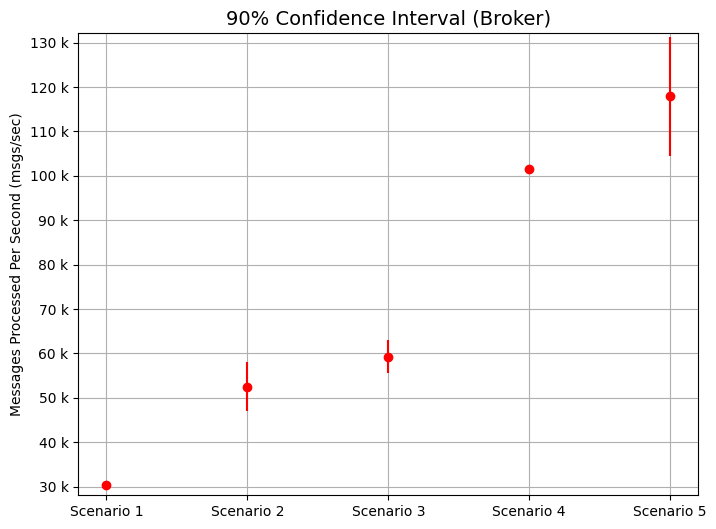
\includegraphics[width=0.75\textwidth]{chapters/images/confidence-intervals/broker-message-ci.png}
    \caption{Broker message throughput confidence interval}
    \label{fig:chapter07:discussion:brokermessageci}
\end{figure}

The boundaries of Scenario 2 and Scenario 3 overlap. A t-test was performed with the resulting p = 0.0673, indicating that the difference between them is not statistically significant. The other scenarios differ from each other significantly, proving that in most cases the performance improved significantly with higher parallelization.

\subsection{Sink Connector}
Figure \ref{fig:chapter07:discussion:sinkmessageci} shows the confidence interval results for the sink connector's message throughput. The boundaries are too narrow to be visible for Scenarios 1-3, possibly due to low throughput variability. This is also supported visually by Figure \ref{fig:chapter06:results:sinkallscenarios} and by comparing the mean and median in Table \ref{tab:kafka:messagethroughputsink}. The boundaries for Scenario 4 and Scenario 5 are higher. However, they are still relatively narrow. This is unexpected for Scenario 5 especially, as it contains very high variability in Figure \ref{fig:chapter06:results:sinkallscenarios} and a very high difference between the mean and median in Table \ref{tab:kafka:messagethroughputsink}. A possible explanation could be similar to that of the broker, as the sink's activity in Scenario 5 was also less than 1.5 minutes, leading to a very small window of measurements.

\begin{figure}[htbp]
    \centering
    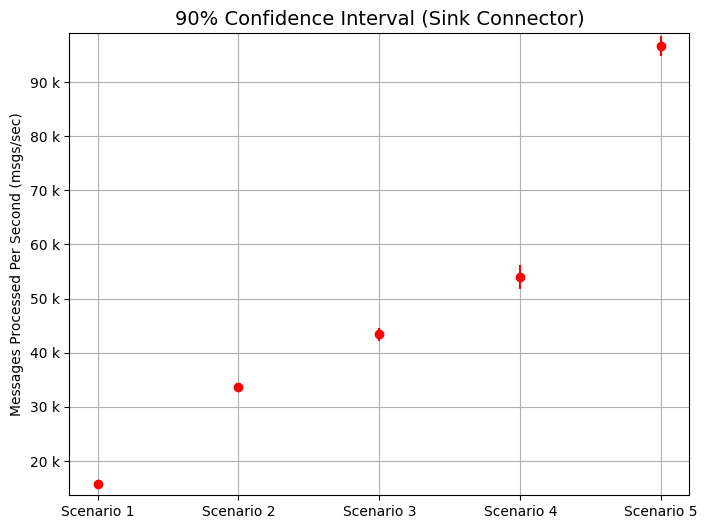
\includegraphics[width=0.75\textwidth]{chapters/images/confidence-intervals/sink-message-ci.png}
    \caption{Sink connector message throughput confidence interval}
    \label{fig:chapter07:discussion:sinkmessageci}
\end{figure}

All of the scenarios are significantly different from each other based on visual evaluation, indicating that parallelization had a statistically significant impact on the performance in all measured scenarios.

\section{Effects of Parallelization}
Overall, the confidence intervals discussed in \ref{ch07:discussion:statsig} showed that the increase in parallelization had a statistically significant impact on the performance of all components in the Kafka replication pipeline. The source connector and the broker experienced the most significant improvement in throughput in Scenario 4, when the same number of tasks that were run in Scenario 3 were distributed on two workers in the source connector. This speaks not only to the positive impact of parallelization, but also to that of distributed processing. The increase in the broker's performance, despite no changes to its configuration, shows that the broker's performance scaled with the source connector. % add screenshots of cpu usage?

The same effect of distribution was not observed for the sink connector. As seen in Figure \ref{fig:chapter07:discussion:sinkmessageci}, the distribution of tasks to an additional worker improved the performance slightly. Nevertheless, the most significant performance increase occurred in Scenario 5, when additional workers and more than double the number of tasks were added to the sink connector. This shows that the sink connector could require a higher degree of parallel processing to achieve similar results to the source connector. However, at approximately 97K messages per second, the sink connector is still below the source connector's performance in Scenario 4 and Scenario 5. This leads to the possibility that the Postgres database is the actual bottleneck, and that latencies related to the upsert operations influence the performance of individual tasks. This would explain why increasing the number of tasks increases the performance more drastically than increasing the number of workers: the more tasks, the more operations can be performed despite connector or database latencies. It would be interesting for further research to investigate whether different database configurations or even different relational databases would affect the sink connector's performance. More testing would also be required to determine the optimal degree of parallelization for the source connector.

Scenario 5 proved to have an unexpected result for the source connector (and, by extension, the broker). It was expected that such a significant increase in tasks and workers would result in a more significant improvement in performance. A possible reason for that could be that the EntireX Broker queue becomes the bottleneck and cannot handle the high number of parallel tasks. A possible solution for that could be to configure multiple queues, each of which is responsible for a certain range of \ac{ISN}s. This would allow for the performance of the EntireX Broker to scale together with the performance of the source connector. It would be interesting to run more tests in the future to determine the load limit of a single EntireX Broker queue and the effect of multiple queues on overall performance.

\section{Scalability and Architectural Considerations}
% very scalable, however increased complexity, need to manage cluster and its health
% mention in prev section that performance bottleneck may exist - then clarify here that scalable up to a certain extent, what else can be done to improve that scalability (multiple queues, more jdbc tasks, etc.)
As the various scenarios have shown, the Kafka replication pipeline is extremely scalable, allowing the degree of parallelization to be increased with ease. However, as discussed in the previous section, there is the possibility of other bottlenecks in the system, such as the EntireX Broker queue and the Postgres database. The EntireX Broker can be scaled, as discussed, by adding additional queues for processing specific \ac{ISN} ranges. With regards to Postgres, the results of Scenario 5 showed that a large number of tasks had a more positive impact on the sink connector's performance. Database query and insertion latency could be the culprit, in which case scaling the sink connector to a greater degree than the source connector could be of benefit. If, however, further scaling of the sink connector does not improve performance, it might be helpful to consider running Postgres as a distributed database. This would allow for Postgres to be scaled along with the Kafka replication and with the EntireX Broker, improving not only scalability but also availability of the database. A possible strategy for scaling Postgres is with Citus, a database engine that allows for Postgres to be run and scaled as a distributed database \cite{cubukcu2021citus}.

Overall, the scalability of the Kafka replication solution is a major advantage compared to \ac{ART}, as it can improve overall performance and guarantee availability. However, as with any distributed system, there is also its complexity to consider. While the performance increase might be beneficial, there is also the maintenance of the Kafka cluster to consider in a production environment. This requires constant monitoring of the cluster's health, especially in case nodes become unavailable or any unknown errors cause tasks to fail and crash. This requires additional resources, not to mention the cost for hosting such a cluster around the clock. It is therefore important to consider whether the additional cost and maintenance effort are worth the required increase in performance and scalability. The Kafka-based solution might be especially attractive for companies with an existing Kafka cluster, since they already have an existing infrastructure and trained specialists to monitor and maintain the entire replication pipeline.

\subsection{The Consistency vs. Performance Trade-off}
As already discussed in \ref{ch04:pipelinedevelopment:parallelizationconsiderations}, parallelization leads to new aspects that have to be considered, such as the balance of consistency, performance, and availability. Unlike \ac{ART}, the Kafka-based solution can lead to unavoidable inconsistencies when running in parallel. As also previously mentioned, a possible solution is to implement Kafka Streams to order messages before they are sent to the sink connector. If there is a one-to-one assignment of sink tasks to Kafka partitions after the Streams transformation, the correct message order can be guaranteed. Unfortunately, modifications to improve consistency can have a negative effect on performance. It is therefore important to consider the requirements of the replication system. If consistency is extremely important, the replication pipeline has to be improved at the possible cost of performance.

\section{Performance Variability}
\label{ch07:discussion:performancevariability}
% variability - different number of transactions/Adabas records per EntireX broker message - partial cause?
% dockerization, garbage collection - drops in performance
% entirex broker and postgres bottleneck?
% multiple reads from entirex broker saturate the network better??
High performance variability was observed in the source and sink connectors, especially in scenarios involving a higher degree of parallelization. The more significant drops in performance can possibly be attributed to garbage collection. As the paper by \citeauthor{cai2022distillinggc} found, garbage collection can incur substantial cost in an application's performance, so it is not to be dismissed when discussing performance \cite{cai2022distillinggc}. The paper is especially relevant, as it examines Java 17, the same version used for the Kafka connectors and \ac{ART}. In the future, it would be beneficial to test the performance of the Kafka replication with various garbage collectors and investigate their effect, if any, on the connectors' performance.
It is also possible that the EntireX Broker's performance was a factor in the performance drops, especially in the later scenarios with a lot of concurrent reads from the message queue. However, the EntireX Broker's performance was outside of the experiment scope. It would be of interest to investigate the EntireX Broker's impact on performance in future experiments.

Regarding the burst pattern of \ac{ART}'s transaction throughput, there were usually approximately 10 transactions processed at a single time with a few seconds of pause in-between. This grouping of transactions is a result of the \ac{REPTOR} message, seein as "replicated data for different transactions may be sent in the same message" \cite{reptorprogrammersref}. As a result, 10 transactions are typically received in one message and processed at a time by \ac{ART}. The pauses in-between could be related to the processing time needed by \ac{ART} before a new message can be read from the message queue. 

Although \ac{ART}'s message throughput also varied, the standard deviation remained relatively constant in Figure \ref{fig:chapter06:results:artavgmessage}. The difference in the mean and median in Table \ref{tab:art:messagethroughput} was also not significant. It can therefore be assumed that the variability in messages processed per second came from the variability of the number of records and their content in each transaction. 

\section{Experiment Limitations}
% only initial state tested for "consistent" results and similarity - interesting how updates would affect, as art doesn't receive full data image
% interesting in future to test flat fields only or more periodic fields
The limitations of connector development and scope were elaborated in \ref{ch04:pipelinedevelopment:solutionlimitations}. Another limitation of the experiment methodology itself is the fact that only the \ac{IS} event was tested for performance. As explained in \ref{ch05:methodology:design:scenarios}, this was due to the upsert nature of the \ac{JDBC} sink connector and for ease of experiment set up, since no records had to be re-created or deleted for every run, while allowing the entire database content to be replicated at once. Another reason was reproducibility, since running the \ac{IS} ensured a consistent structure of the produced \ac{REPTOR} messages, such as the number of transactions in each message. In future investigations, it would be of interest to investigate whether insert or update operations have a difference in performance, as \ac{ART} does not support the upsert strategy. A further test idea would be to investigate how the performance is affected by the complex Adabas data structures. This would involve running tests with Adabas records containing only flat fields, as well as records containing a higher variety of complex and nested data structures than was available in the current experiment.